\documentclass[twoside=semi,fontsize=12pt,paper=a4,titlepage=on]{kv_article}
%\documentclass[twoside=true,fontsize=12pt,paper=a4,titlepage=off]{article}
\usepackage{graphicx}
\usepackage{amssymb, amsmath, bm}
\usepackage{multirow}
\usepackage{mathtools}
\usepackage{array}
\usepackage{enumitem}
\usepackage{arydshln}
\usepackage{subfig}
\usepackage{tabularx}
\usepackage{xurl}

\begin{document}

\title{Can RFI in Ny-Ålesund be detected in the VLBI data analysis?}
\subtitle{\vspace{1cm}Case study: Ny-Ålesund and Wettzell}
%{\vspace{2cm}Norwegian Mapping Authority}
\author{Ann-Silje Kirkvik}
\date{\today}

\maketitle

\section{Background}
In Ny-Ålesund Research Station there are restrictions on the use of radio frequencies (RF) in the frequency range 2-32 GHz in the geographical area within a 20 km radius from Ny-Ålesund \cite{nyalesundresearch}. This restriction is set up to protect the VLBI observations and is enforced by law. Due to the increasing amount of electronic devices that use Wi-Fi and Bluetooth this legislation is under pressure.

This report is a quick study to see if the radio frequency interference (RFI) can be detected in the VLBI data analysis. If the results of a VLBI session are not optimal there are usually numerous sources of potential issues and it will be very difficult to attribute the lack of performance to local RFI specifically. For instance, a VLBI observation consists of a pair of VLBI stations and a radio source (quasar). Either of these three components may not behave as expected and impact the analysis results. A station may have technical issues and a quasar can have time variable source structure that is not modelled in the data analysis.

Even there if there is a legislation in place to prohibit RFI, it is very hard to enforce this legislation and there are almost always some transmitting devices that are not turned off. The Ny-Ålesund Research Station is an isolated science community with a small population in the winter season and with many visiting researchers in the summer season. In addition, the cruise ships primarily travel to Ny-Ålesund between June and August. The idea is therefore to investigate if there is a seasonal signal in the performance at the station NYALES20. Figure \ref{fig:nyal_map} shows a map of Ny-Ålesund and the surrounding area, including the station NYALES20 and the new stations NYALE13S and NYALE13N.

\begin{figure}[htpb!]
\centering
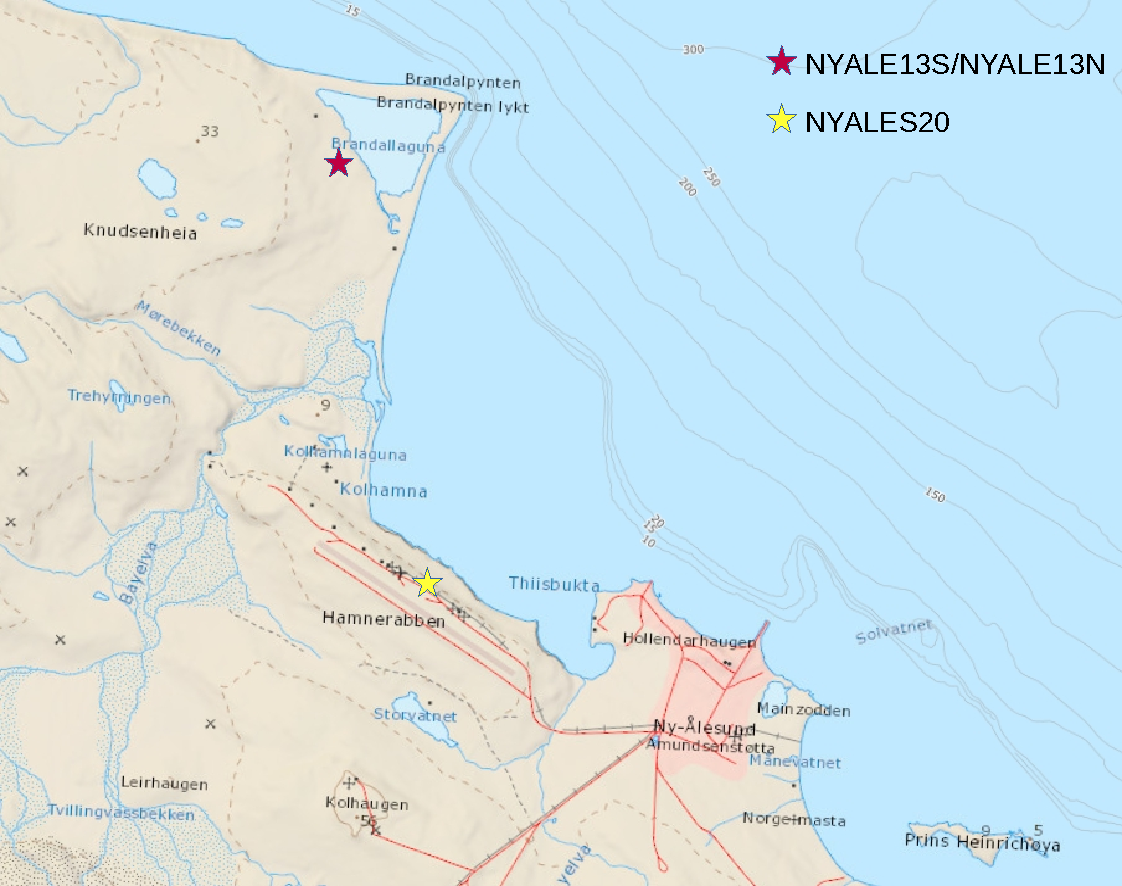
\includegraphics[width=\linewidth]{fig/Nyal_map.pdf}
\tiny Made from https://experience.arcgis.com/experience/543df24b254a47d2951f462010c42b91
\caption{Map of Ny-Ålesund and surrounding area. The distance from the village to NYALES20 is approximately 1.3km and the distance between NYALES20 and NYALE13S/NYALE13N is approximately 1.5km. The height of the village is around 7-8m and the height at NYALE13S/NYALE13N is around 6m. NYALES20 is higher in the terrain around 40m.}
\label{fig:nyal_map}
\end{figure}

There are already many seasonal signals in VLBI data. Some of these signals are accounted for in the data analysis and some are not. Even if a seasonal signal is detected it can not necessarily be attributed to local RFI. Regardless, an attempt is made to do this investigation and it is therefore useful to compare with another station that is not expected to have signification seasonal variations in RFI. For this purpose the comparison will be done with the WETTZELL station.
  

\section{Data and Method}
%%\label{sec:data_and_method}
One application of VLBI data is the realization of the International Terrestrial Reference Frame  (ITRF) \cite{altamimi2023}. In the beginning of 2026 a full reprocessing of all historic 24 hour VLBI sessions up until 31st of December 2025 was done in preparation for the next ITRF update, namely ITRF2020-u2025. This analysis is done independently by multiple analysis centers and this report uses the output from the analysis done by the Norwegian Mapping Authority (NMA) analysis center. 

The ITRF is realized by combining data from multiple geodetic techniques, namely VLBI, SLR, DORIS and GNSS. To ensure consistent modelling across the different techniques a set of conventions has been developed. The current convention is the IERS 2010 conventions \cite{iers2010}. The dataset used in this analysis follows these conventions. The conventions describe, including, geophysical models for intraday station displacements and variations in Earth Orientation Parameters (EOP). These models include, for instance, the solid earth tides (movement of the earth crust) due to gravitational forces from the Sun and the Moon. There are, however, several geophysical models that are not included in the conventions. One example is the non tidal atmospheric loading and ocean loading. These models have a seasonal signal and is expected to impact the estimated station coordinates \cite{wang2025}. This report will not look into the estimated station coordinates. It will focus on the post fit residuals after the data analysis. These residuals may contain traces of unapplied models even if the effects should in theory transfer to the estimated station coordinates. 

\subsection{Data selection}
The dataset consist of 7716 sessions. Since these sessions were originally analyzed with a ITRF realization in mind, sessions with a network volume less than 10Mm$^3$ are discarded. This selection criteria was also used in for the ITRF2020 realization \cite{altamimi2023}. 

Individual stations that successfully participated in less than 50 sessions are also not considered when looking into seasonal signals. If at least some observations from a station are used in the final analysis the station is considered to have participated successfully. Figure \ref{fig:num_sessions} shows the number of successful sessions for each station. Notably, NYALES20 and WETTZELL are among the top contributors in the history of geodetic VLBI. WETTZELL started observing in 1983 and is still operational. NYALES20 started observing in 1994 and was decommissioned in 2023. The co-located stations NYALE13S and NYALE13N in Ny-Ålesund and WETTZ13N and WETTZ13S in Wettzell are not investigated in this study due to shorter observation history. % Show some plots in appendix?

\begin{figure}[htpb!]
\centering
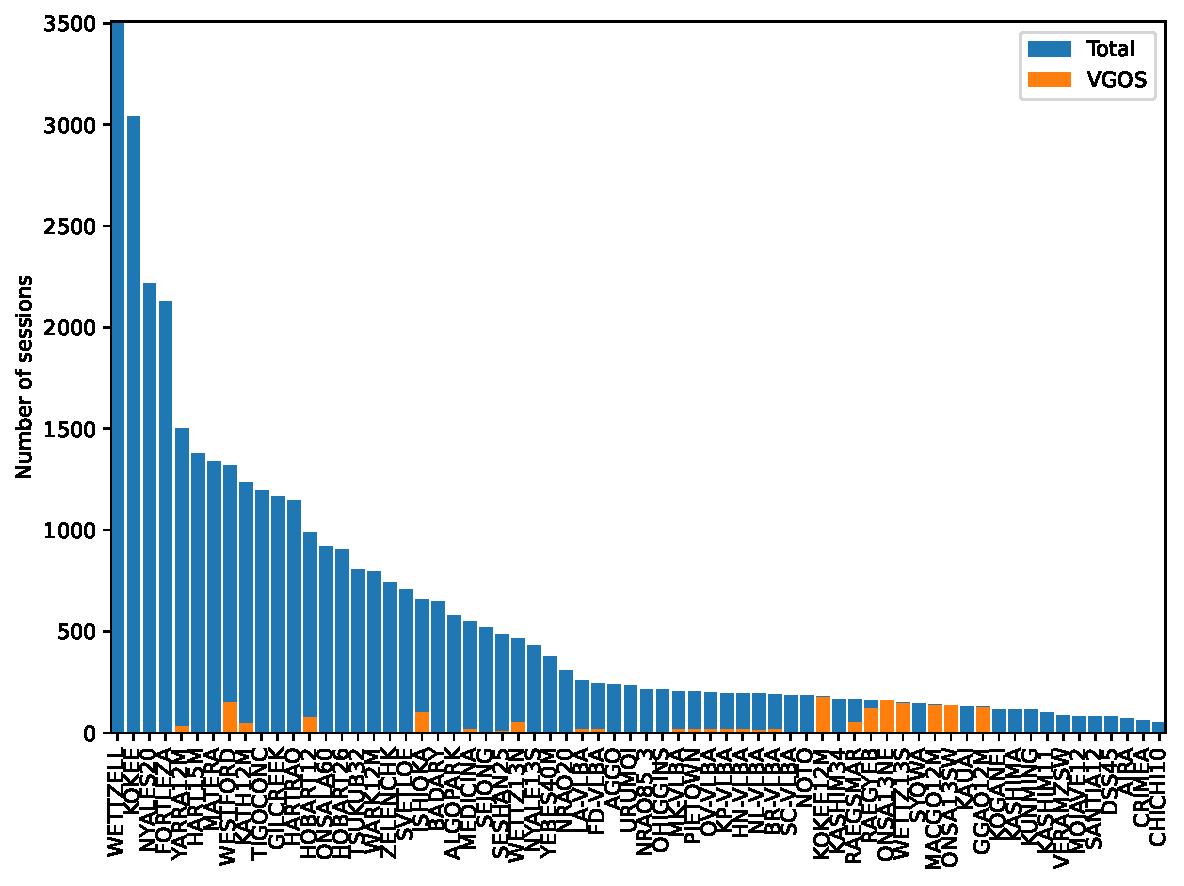
\includegraphics[width=\linewidth]{fig/Number_of_sessions.pdf}
\caption{Total number of 24 hour sessions (blue) and VGOS sessions (orange) the VLBI stations have successfully participated in from 1979 to 2025. There is a cutoff at 50 sessions.}
\label{fig:num_sessions}
\end{figure}

Figure \ref{fig:residuals} shows the Root Mean Square (RMS) of the post fit residuals for NYALES20 and WETTZELL, respectively, that will be used in this report. On average, the the RMS is expected to be around 1cm for legacy S/X sessions. For NYALES20 there seems to be a increase in residuals some time after 2020. This is most likely due to numerous technical problems at the station at the end of its lifetime. See for instance \cite{kirkvik2021} and \cite{garciaespada2023}. NYALES20 was planned for decommissioning by 2020, but the lifetime was extended to try to get more parallel observations with the NYALES13S antenna that saw first light in 2020. 

\begin{figure}[htpb!]
\centering
\subfloat[\textcolor{black}{NYALES20}.\label{fig:residual_ny}]
	{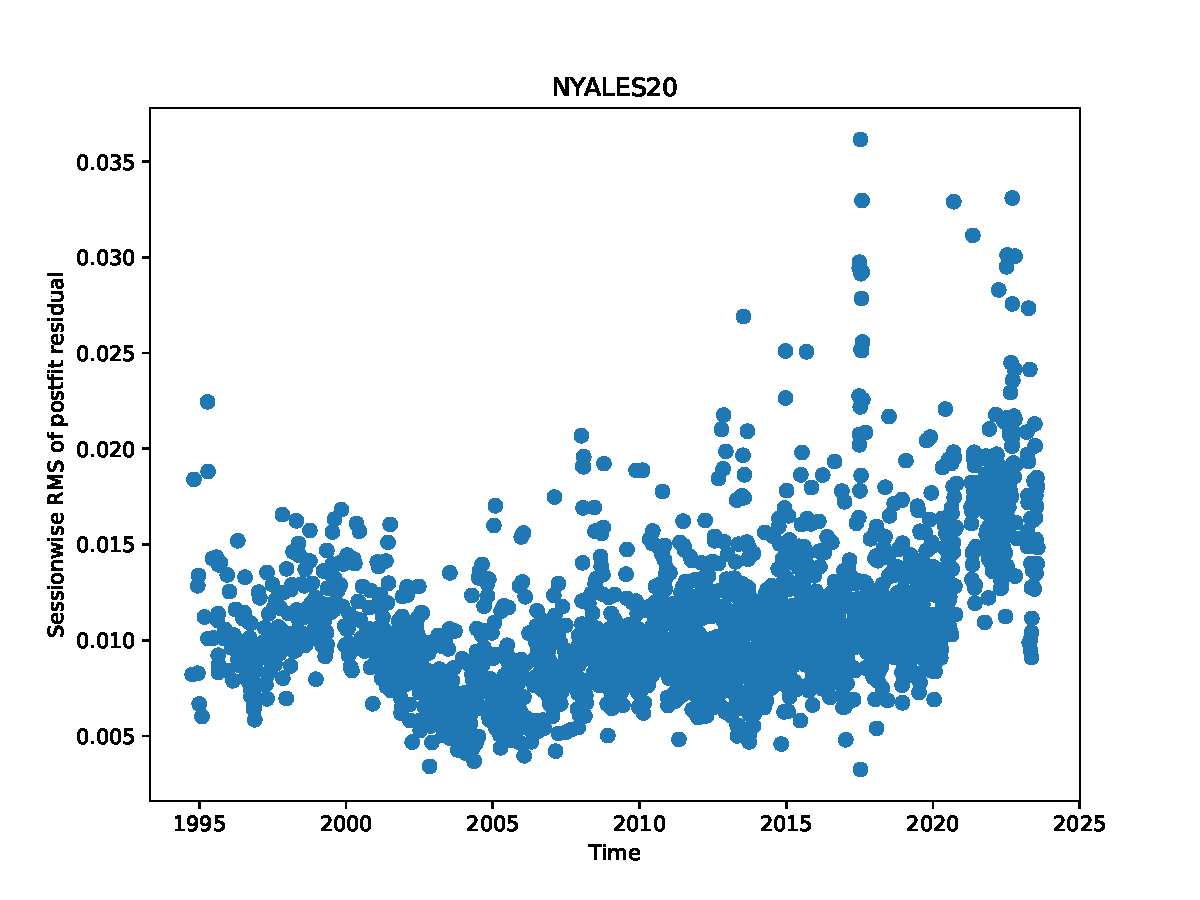
\includegraphics[width=0.5\linewidth]{fig/Residual_NYALES20.pdf}}
\subfloat[\textcolor{black}{WETTZELL}.\label{fig:residual_wz}]
	{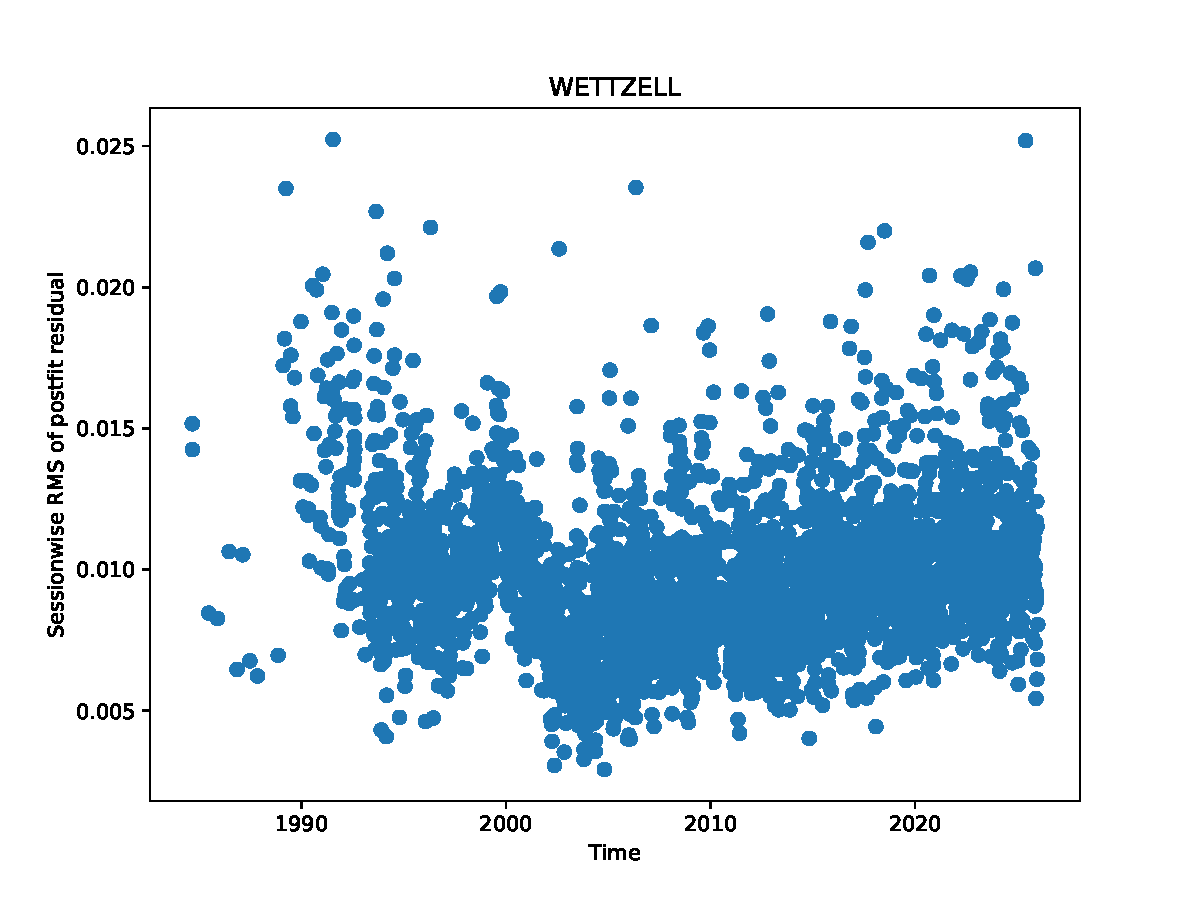
\includegraphics[width=0.5\linewidth]{fig/Residual_WETTZELL.pdf}} \\
\caption{RMS of post fit residuals for a station for each session.}
\label{fig:residuals}
\end{figure}
%ITRF2020-u2025 submission
%geophysical models / station displacement models: 
%ocean loading
%solid earth tides
%+++
%examples of missing models:
%non tidal atmospheric loading
%hydro-something? 

%Data selection:
%Stations defined in ITRF2020
%Networks lager than 10Mm**3
%More than 50 sessions
\subsection{Data analysis}

Several aspects of the residuals have been investigated to look for impact from RFI. The session performance have also been considered to some degree.

\subsubsection{Monthly performance}
A VLBI session is based on a schedule. The schedule tells a station when to observe, where to point in the sky and for how long. The schedule consists for multiple such planned observations for multiple stations. When the data is recorded at a station it is sent to a central correlator which will combine the data with other stations. If the correlator is able to successfully correlate two datasets an observation is computed for that pair of stations and the observed quasar. These observations are then analysed further to obtain the desired output. Unusable or bad observations are discarded from the final analysis. To see if there is a seasonal dependence in the number of observations that are usable in the analysis compared to the planned observations, the number of scheduled, correlated and used observations are stacked for each month. Since a plan can vary from month to month a normalized version is also computed.    

\subsubsection{Azimuth dependence?}
Looking at the map in figure \ref{fig:nyal_map}, the Ny-Ålesund village is located east and southeast of NYALES20. There is an open sea/fjord to the north and mountains to the west and south. RFI will mostly come from the village and possibly from boats. This raises the question of whether the residuals are higher when the antenna is pointing towards the city and lower when pointing towards (and above) the mountains. This is checked by looking at the correlation between the residuals and the azimuth angle of the observations.

\subsubsection{Spectral analysis}
When looking for a seasonal signal in a dataset it is common to do a spectral analysis. A very common method is to do a Fourier transform and investigate the data in the frequency domain. However, the Fourier approach assumes that the data is evenly spaced. That is not the case for VLBI data. For unevenly spaced data the Lomb-Scargle Periodigram is commonly used \cite{vanderplas2018}. For this report the implementation of this algorithm from astropy\footnote{https://docs.astropy.org/en/latest/timeseries/lombscargle.html} was used. The frequencies that were investigated corresponds to periods from 30 to 1200 days. If there is a strong annual signal in a dataset there is expected to be a high peak in the Lomb-Scargle Periodigram at 365.25 days.

\section{Results}
The results from the three different investigations are summarized here. 

\subsection{Monthly performance}
The monthly performance is shown in figure \ref{fig:monthly}. As can be seen in the left column, the number of scheduled observations clearly vary from month to month. There are many explanations for this. There may be periods when more sessions are planned, for instance during a CONT-campaign. A CONT-campaign is typically daily sessions for 14 consecutive days while there are 2-4 sessions per week normally. August is typically the month when NYALES20 is taken offline for about a week to perform maintenance. When a station cannot participate in a session as planned the schedule may be remade without that station if the scheduler is notified in time (typically at least one week before). For prolonged outages the station is then usually removed from the upcoming schedules. 

The right column that shows the normalized monthly performance have less variability and should be easier to interpret. At WETTZELL the performance seem stable throughout the year, while there is more variability at NYALES20. This could be because WETTZELL have a longer observation history and that the results are more averaged out over the years. However, looking only at 1994-2023 for WETTZELL (not shown) gives the same impression as in figure \ref{fig:monthly_wz_norm}. July is the month with the worst performance for NYALES20 and RFI cannot be excluded as a factor, but the difference from January is not very large and makes any conclusions difficult.

\begin{figure}[htpb!]
\centering
\subfloat[\textcolor{black}{NYALES20}.\label{fig:monthly_ny}]
	{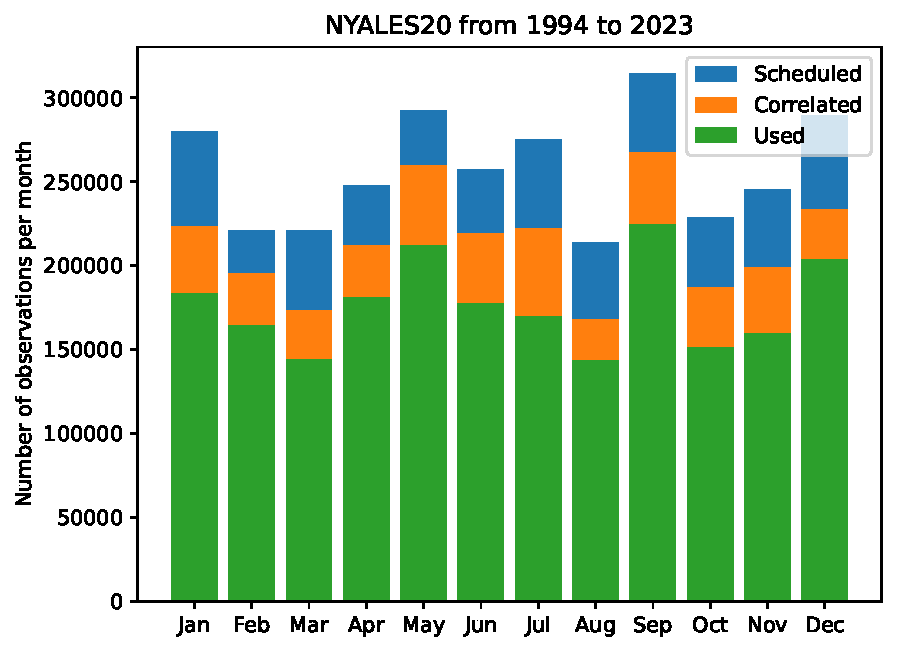
\includegraphics[width=0.5\linewidth]{fig/Num_obs_per_month_NYALES20_1994_2023_2025b.pdf}}
\subfloat[\textcolor{black}{NYALES20 normalized}.\label{fig:monthly_ny_norm}]
	{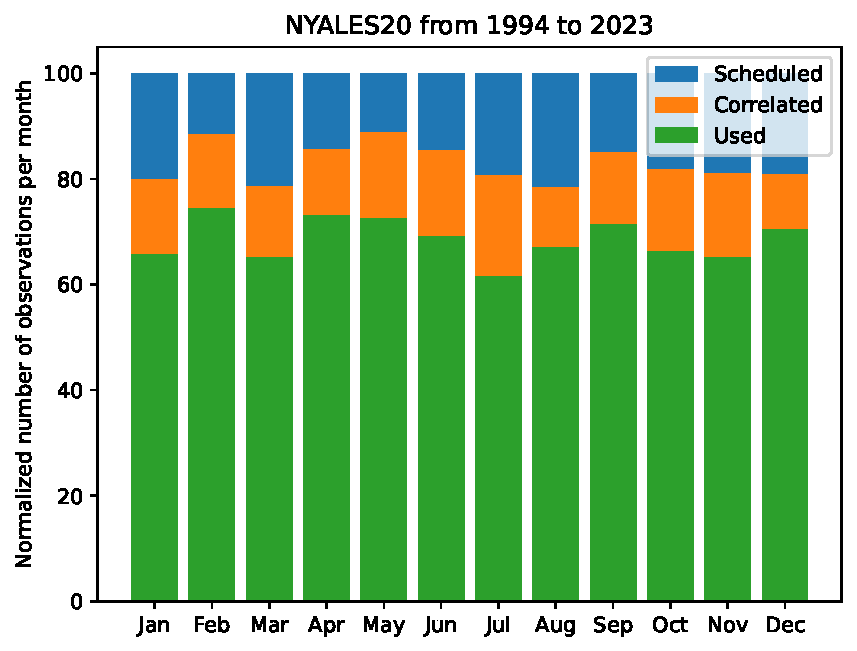
\includegraphics[width=0.5\linewidth]{fig/Num_obs_per_month_NYALES20_normalized_1994_2023_2025b.pdf}} \\
\subfloat[\textcolor{black}{WETTZELL}.\label{fig:monthly_wz}]
	{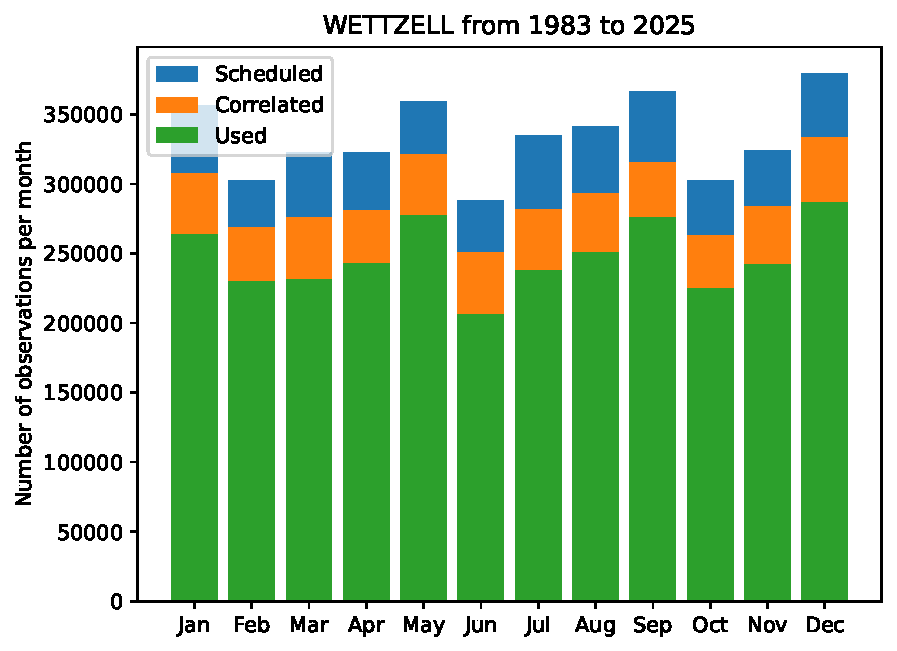
\includegraphics[width=0.5\linewidth]{fig/Num_obs_per_month_WETTZELL_1983_2025_2025b.pdf}}
\subfloat[\textcolor{black}{WETTZELL normalized}.\label{fig:monthly_wz_norm}]
	{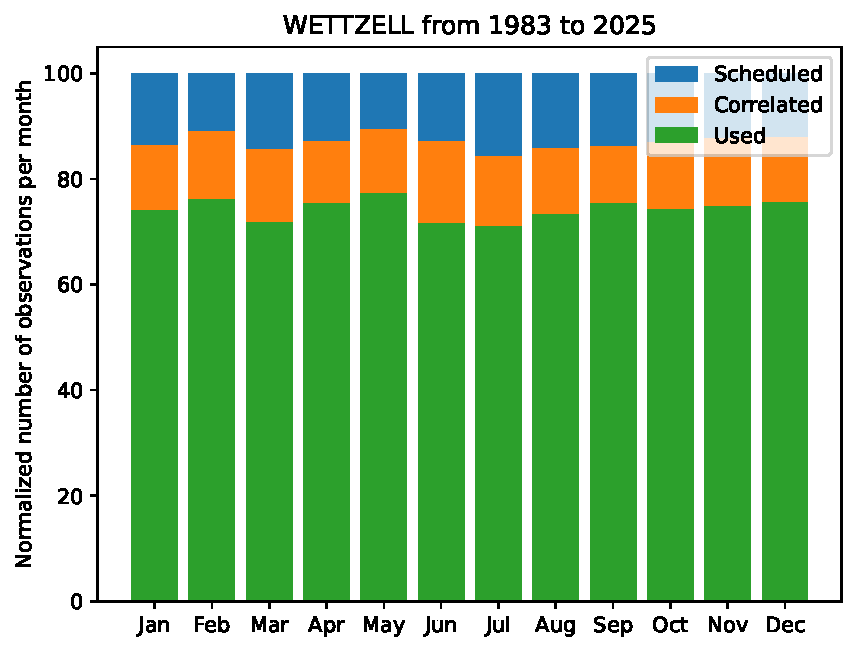
\includegraphics[width=0.5\linewidth]{fig/Num_obs_per_month_WETTZELL_normalized_1983_2025_2025b.pdf}} \\
\caption{The left column shows the number of scheduled, correlated and used observations for NYALES20 (\ref{fig:monthly_ny}) and WETTZELL (\ref{fig:monthly_wz}) for each calendar month. The left column shows the normalized version for NYALES20 (\ref{fig:monthly_ny_norm}) and WETTZELL (\ref{fig:monthly_wz_norm}). Here 100 means all scheduled observations. NYALES20 have an observation period of 29 years, while WETTZELL have an observation period of 42 years.}
\label{fig:monthly}
\end{figure}

\subsection{Azimuth dependence?}

Figure \ref{fig:skyplot_ny} shows how the absolute value of the residuals of the individual observations are distributed in the sky over the station. For this plot the residuals from one year of observations are accumulated. In total there are 94603 data points. The year 2020 was picked arbitrary and picking another year gives similar results (not shown). There is no indication from visual inspection that the residuals are higher in any specific direction. This is emphasized further in \ref{fig:res_vs_az_ny} were the residuals are plotted with regards to azimuth angle. The computed Pearson correlation coefficient is -0.0073, which means there is no correlation between the residual and the azimuth angle.
%2025b: Number of observations total for NYALES20: 94603
%2025b:The correlation coefficient (r) between residuals and azimuth for NYALES20 is: -0.007336549154459748
%2025b:The p-value is: 0.024036392681316323
%2025b:The correlation coefficient (r) between residuals and elevation for NYALES20 is: 0.0005374500621803742
%2025b:The p-value is: 0.8687042606100198

\begin{figure}[htpb!]
\centering
\subfloat[\textcolor{black}{NYALES20 2020}.\label{fig:skyplot_ny}]
	{\includegraphics[width=0.5\linewidth]{fig/Skyplot_NYALES20_2020\-01\-01_2020\-12\-31_2025b.pdf}}
\subfloat[\textcolor{black}{Absolute value of residual vs Azimuth}.\label{fig:res_vs_az_ny}]
	{\includegraphics[width=0.5\linewidth]{fig/Residual_vs_Azimuth_NYALES20_2020\-01\-01_2020\-12\-31_2025b.pdf}} \\
\caption{Skyplot with absolute value of residuals for individual observations for NYALES20 for the year 2020 (\ref{fig:skyplot_ny}). Darker color implies higher residual. The colorbar is capped at 10cm. The same residual plotted with regards to the azimuth angle (\ref{fig:res_vs_az_ny}). The computed Pearson correlation coefficient is -0.0073, indicating no correlation.}
\label{fig:skyplot}
\end{figure}

\subsection{Spectral analysis}

Figure \ref{fig:ls} shows the output of the Lomb-Scargle Periodigram algorithm. An annual signal should have a significant peak coinciding with the red vertical line. In figure \ref{fig:ls_ny} there is a peak close to this line, but it is not very high compared to other peaks. The peak is also fairly wide. The periodigram indicates that there may be an annual signal, but the results is very noisy. The same plot is shown for WETTZELL in \ref{fig:ls_wz}. Here, the peak is much clearer and there is also a clearer small peak at the semiannual period. The most likely explanation is unmodelled geophysical effects. Since the seasonal signal is stronger in WETTZELL than in NYALES20 it seems unlikely that seasonal variations in the population in Ny-Ålesund is the cause of any seasonal signal in NYALES20. 

To see if there is any geographical implications in the annual and semiannual peaks the output from the Lomb-Scargle Periodigram algorithm closest to the annual and semiannual period is selected for each station and plotted on a map in figure \ref{fig:ls_map}. The station with the largest annual peak is the Japanese station SYOWA in Antarctica. A natural assumption is that this could be related to unmodelled geophysical effects due to melting ice, but this has not been investigated further. NYALES20 is known to have a non-linear and increas uplift due to melting ice cite{kierulf2021}, \cite{kierulf2026}. There is no proper model for this effect in the analysis, but there is a discontinuity in the station velocity in the ITRF2020-u2023 and later updates at at the epoch 2016.0 to somewhat compensate for this effect. The other stations on the map seem to be fairly close in value, which can also be gleamed from the periodigram plots. The station with the largest semiannual peak is the US station MACGO12M. This is a relatively new station VGOS station that started observing in 2020. The second largest peak is KOKEE12M and the third is GGAO12M. As can be seen in \ref{fig:num_sessions}, all these stations have participated in relatively few sessions and mostly VGOS session. These peaks are in general very low and might be false detections. On the other hand VGOS sessions are expected to perform better than legacy S/X sessions and maybe geophysical signals might be easier to detect for this session type. 

\begin{figure}[htpb!]
\centering
\subfloat[\textcolor{black}{NYALES20}.\label{fig:ls_ny}]
	{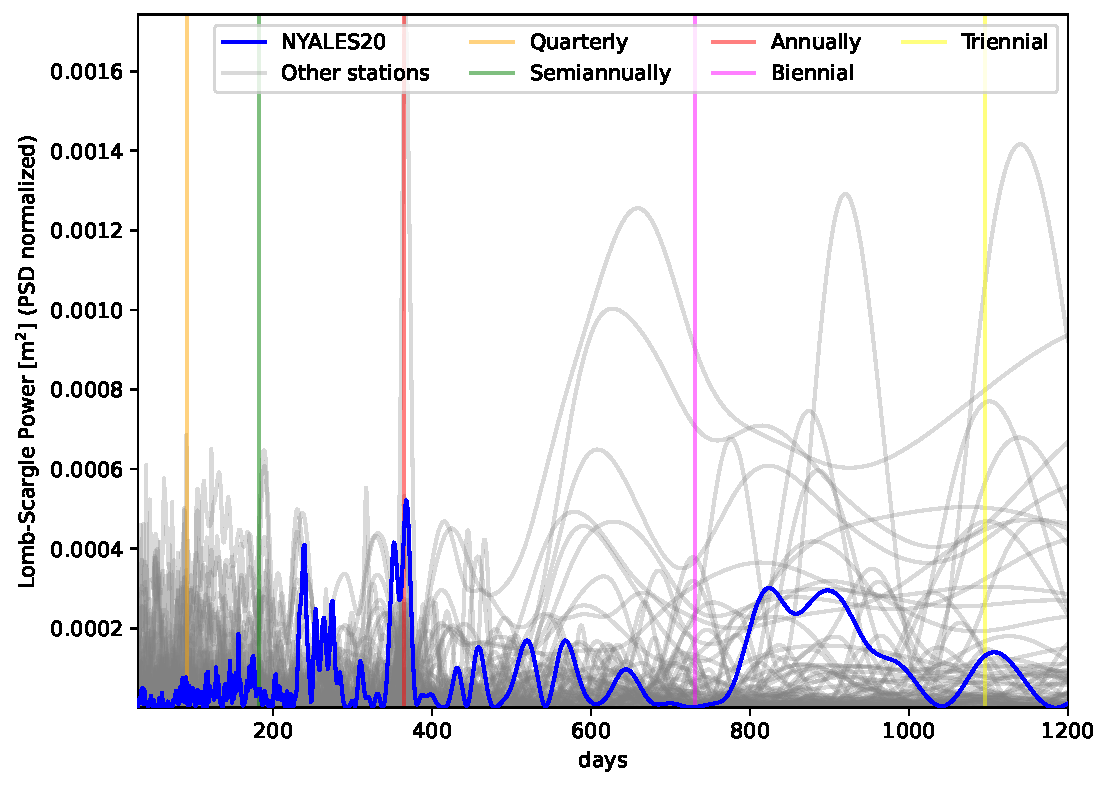
\includegraphics[width=0.5\linewidth]{fig/LombScargle_power_NYALES20.pdf}}
\subfloat[\textcolor{black}{WETTZELL}.\label{fig:ls_wz}]
	{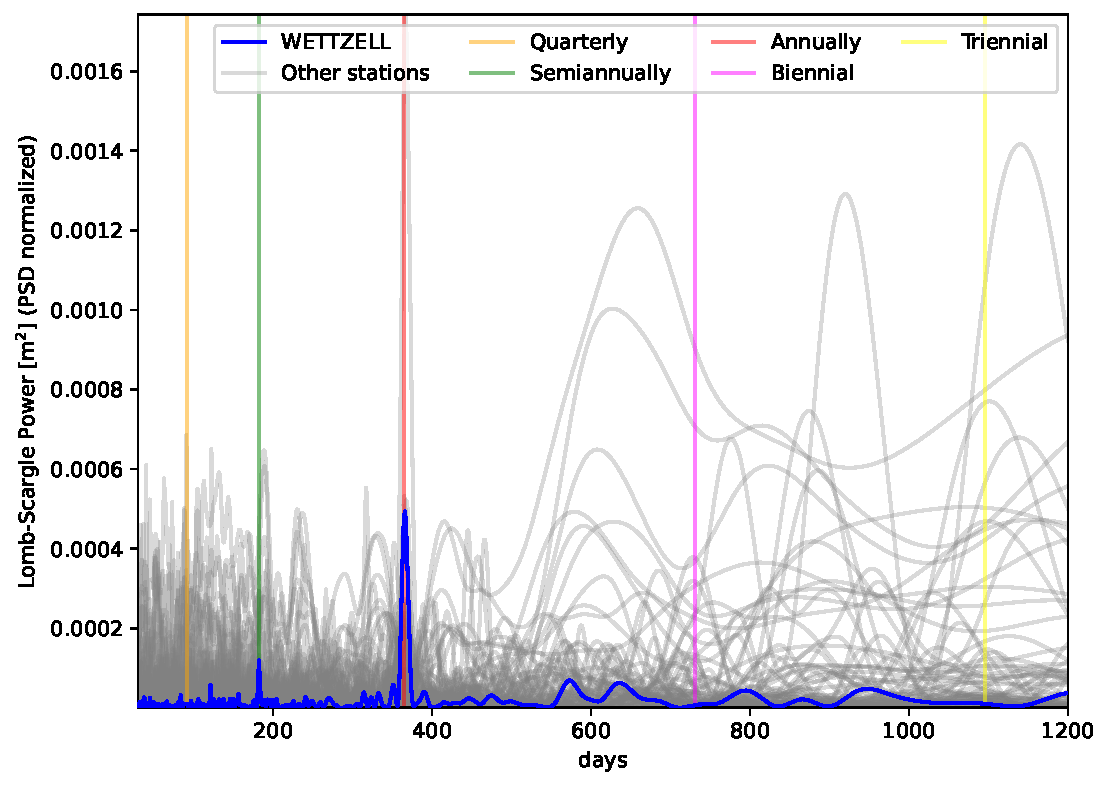
\includegraphics[width=0.5\linewidth]{fig/LombScargle_power_WETTZELL.pdf}}
\caption{Lomb-Scargle periodigram with power spectrum density (PSD) normalization for all stations (gray) with more than 50 successful sessions. The result for NYALES20 (\ref{fig:ls_ny}) and WETTZELL (\ref{fig:ls_wz}) is highlighted in blue. Vertical lines indicate different periods from quarterly to triennial.}
\label{fig:ls}
\end{figure}

\begin{figure}[htpb!]
\centering
\subfloat[\textcolor{black}{Annual peak}.\label{fig:ls_annual_peak}]
	{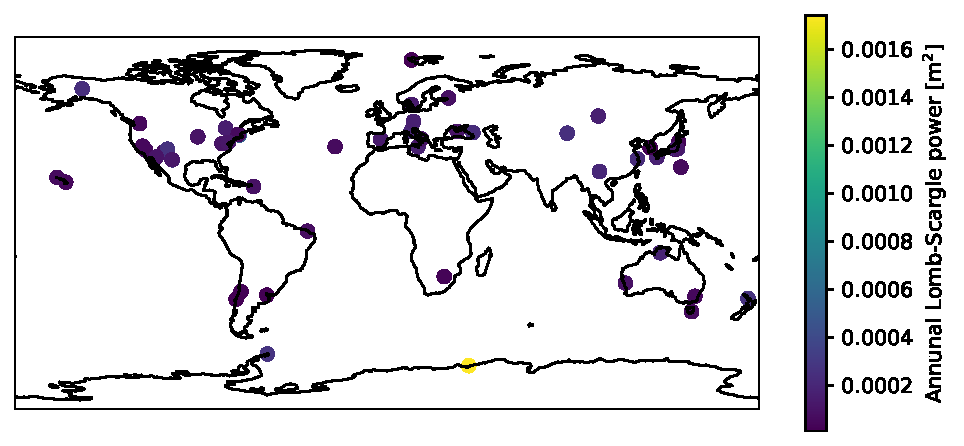
\includegraphics[width=\linewidth]{fig/LombScargle_one_year_power.pdf}} \\
\subfloat[\textcolor{black}{Semiannual peak}.\label{fig:ls_semiannual_peak}]
	{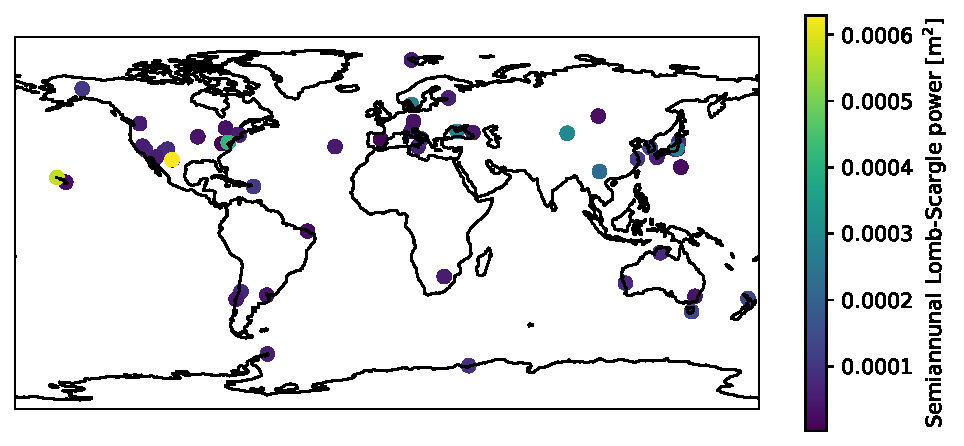
\includegraphics[width=\linewidth]{fig/LombScargle_half_year_power.pdf}}
\caption{The peak close to the annual (\ref{fig:ls_annual_peak}) and semiannual (\ref{fig:ls_semiannual_peak}) signal of the Lomb-Scargle Periodigram for each station. The largest annual peak is found for the Japanese station SYOWA in Antarctica. The largest semiannual peak is found for the US station MACGO12M.}
\label{fig:ls_map}
\end{figure}
 

\section{Conclusions and future work}
% NYALE13S/NYALE13N høyde: 6m, Village: 7~8m. NYALES20:40m % from https://toposvalbard.npolar.no/
There are no clear indications that RFI can be identified by looking at the post fit residuals of a VLBI analysis. There is nothing to indicate a seasonal signal due to RFI at NYALES20. These results, however, cannot be automatically transferred to other stations. This report investigated the station NYALES20 because it has a long observation history. But, since this station was decommissioned in 2023 it is more useful to understand how RFI impacts the newer stations NYALE13S and NYALE13N.

As indicated by the map \ref{fig:nyal_map} the newer stations are lower in the terrain and approximately at the same altitude as the village. These new stations may observe RFI that was not detected at NYALES20. The low noise amplifiers (LNA) in the receivers have already been destroyed a few times in NYALE13S due to boat radar \cite{perez2019} and as a consequence never observes below 15$^\circ$ elevation any longer. NYALES20 never had this issue.

NYALES20 also had a traditional S/X receiver equipped that typically observed in a frequency range around 2.3Hz (S-band) and 8.5GHz (X-band). Going forward NYALE13S and NYALE13N have a VGOS receiver equipped that can observe the whole range from 2-14GHz. The new receiver type may therefore be sensitive to RFI at additional frequencies. 

\subsection{Possible future work}
To eliminate geophysical effects in the spectral analysis more models needs to be applied in the analysis. Most of these models would need to be implemented first. However, this is probably not worth the effort for RFI investigation purposes alone. Even if there is a seasonal RFI signal at NYALES20, the same signal is not expected at the other stations in the global network and the method would not be applicable anywhere else.

The VLBI analysis could be redone and forcebly use all observations from the correlator. I.e. including all the `orange` observations in \ref{fig:monthly}. This will most likely degrade the solution itself, but the residuals might contain some new informations. Maybe the azimuth dependance could be revisted for a small sample size.

The correlator also creates a correlation report with informations about the number of detections and the quality of the detections. Accumulating statistics from these reports might prove some insights. 

For the future the focus should also be on VGOS stations. For these stations longer observation periods are desired if  spectral analysis should be used further. 

\newpage
\bibliographystyle{../../where}
\bibliography{../../where}

\end{document}
